\documentclass[a4paper,12pt]{ctexart}
\usepackage{amsmath}
\usepackage{color}
\usepackage[top=25mm,bottom=25mm,left=20mm,right=20mm]{geometry}
\usepackage{graphicx}
\usepackage{pdfpages}% 直接插入pdf的宏包
\usepackage[colorlinks,linkcolor=red]{hyperref}
\renewcommand\thefigure{\thesection.\arabic{figure}}
\usepackage[superscript]{cite}
\bibliographystyle{unsrt}
\numberwithin{equation}{section}
\graphicspath{{pictures/}}
\author{李玉轩}
\title{BdG方程求解代码编写}
\begin{document}
\maketitle
%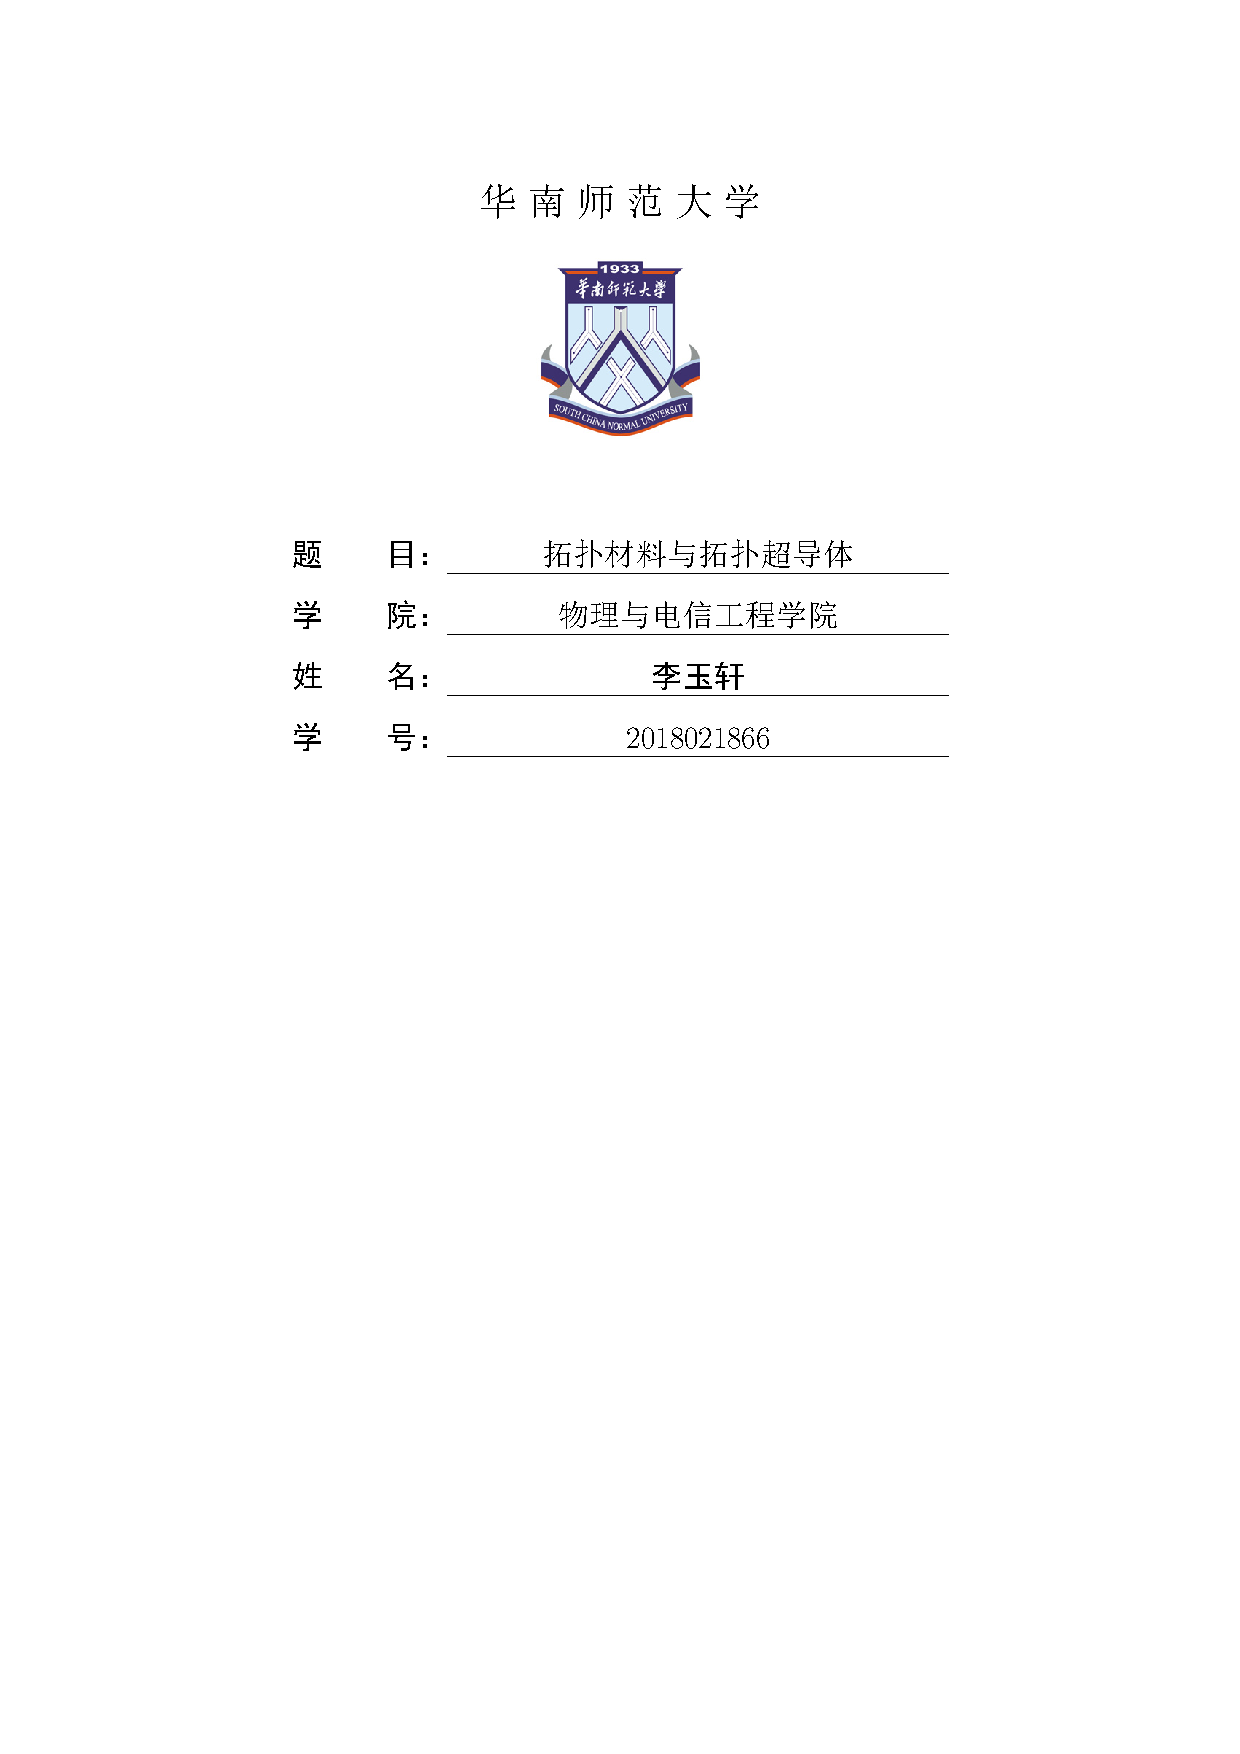
\includepdf{cover/cover.pdf}
\newpage
%\tableofcontents
\section{文档说明}
本手册用来记录在重复论文中遇到的问题,以及计算程序编写过程中,物理公式与程序语言之间的转换关系。本文档所有的代码均已上传至\href{https://github.com/yxli8023/BdG}{GitHub},在使用代码之前,请先阅读\textbf{ReadMe}文件,其中亦有作者的邮箱,欢迎讨论。
\section{模型建立}
代码是用来重复\href{https://github.com/yxli8023/BdG/blob/master/article/PhysRevB.96.184508.pdf}{Vortex pinning by the point potential in topological superconductors:A scheme for braiding Majorana bound states}中的数值结果,其中主要的模型内容如下所示:
\begin{equation}
H = H_t+H_{SO}+H_{SC}
\end{equation}
\begin{equation}
H_t = -\sum_{<ij>}t_0\Phi_{ij}(c_{i\sigma}^\dagger c_{j\sigma}+H.c)+\sum_{i\sigma}(\sigma h-\mu)c_{i\sigma}^\dagger c_{i\sigma}+\sum_\sigma V_ic_{i_0\sigma}^\dagger c_{i_0\sigma}\label{eqhop}
\end{equation}
\begin{equation}
H_{SO}=\sum_{i}(i\lambda\Phi_{ij} c_{i\uparrow}^\dagger c_{i+\hat{x}\downarrow}+i\lambda\Phi_{ij} c_{i\downarrow}^\dagger c_{i+\hat{x}\uparrow}+H.c.
+\lambda\Phi_{ij}c_{i\uparrow}^\dagger c_{i+\hat{y}\downarrow}
-\lambda\Phi_{ij}c_{i\downarrow}^\dagger c_{i+\hat{y}\uparrow}+H.c.)\label{eqsoc}
\end{equation}
\begin{equation}
H_{SC}=\sum_i(\Delta_{ii}c_{i\uparrow}^\dagger c_{i\downarrow}^\dagger+H.c.)
\end{equation}
\begin{equation}
\sum_j 
\left[
\begin{array}{cccc}
H_{ij\uparrow\uparrow}&H_{ij\uparrow\downarrow}&\Delta_{jj}&0\\
H_{ij\downarrow\uparrow}&H_{ij\downarrow\downarrow}&0&-\Delta\\
\Delta_{jj}^\star&0&-H_{ij\downarrow\downarrow}^\star&-H_{ij\downarrow\uparrow}^\star\\
0&-\Delta_{jj}^\star&-H_{ij\uparrow\downarrow}^\star&-H_{ij\uparrow\uparrow}^\star
\end{array}
\right] \Psi_j^\eta=E_\eta\Psi_j^\eta\label{eq:5}
\end{equation}

where  $\Psi_j^\eta=(u_{j\uparrow}^\eta,u_{j\downarrow}^\eta,v_{j\downarrow}^\eta,v_{j\uparrow}^\eta)^T$and$\Delta_{jj}=\frac{V}{2}\sum_\eta u_{j\uparrow}^\eta v_{j\downarrow}^\eta\tanh(\frac{E_\eta}{2K_BT})$
$\sigma$代表自旋取向,向上为1向下为-1,$t_0$代表电子在相邻格点跳跃((hopping)时的能量,$\lambda$代表相邻格点之间的自旋轨道耦合(SOC)强度,$\Delta$是每个格点上不同自旋取向电子的配对能,$\mu$是体系的化学势,求和中的i是格点位置索引,公式中的i代表虚数单位。

通过模型建立,可以得到关于哈密顿量的矩阵形式,模型求解的关键点在于如何通过一系列的公式,正确的写出哈密顿量的矩阵形式,即就是方程(\ref{eq:5})中的矩阵。
\subsection{分析}
\begin{equation}
H=\sum_i(c_{i\uparrow}^\dagger,c_{i\downarrow}^\dagger,c_{i\downarrow},c_{i\uparrow}) \left[
\begin{array}{cccc}
H_{ij\uparrow\uparrow}&H_{ij\uparrow\downarrow}&\Delta_{jj}&0\\
H_{ij\downarrow\uparrow}&H_{ij\downarrow\downarrow}&0&-\Delta\\
\Delta_{jj}^\star&0&-H_{ij\downarrow\downarrow}^\star&-H_{ij\downarrow\uparrow}^\star\\
0&-\Delta_{jj}^\star&-H_{ij\uparrow\downarrow}^\star&-H_{ij\uparrow\uparrow}^\star
\end{array}
\right](c_{i\uparrow},c_{i\downarrow},c_{i\downarrow}^\dagger,c_{i\uparrow}^\dagger)^T
\end{equation}\label{eq6}
\subsubsection{hopping项}
在模型求解过程中,主要是通过建立BdG方程,通过该方法可以实现矩阵的对角化,同时可以得到相应的本征值和本征矢量。从模型的建立来看,主要是通过紧束缚近似的离散晶格模型来构造哈密顿量,在紧束缚近似中,仅仅考虑了每个格点和相邻位置的跳跃和耦合,则可以明白\textbf{公式中的i和j仅仅代表的是最近邻格点位置},即就是$H_{i,j}$可能的形式为$H_{x,x\pm1}$和$H_{i,x\pm y}$,在将哈密顿量写成矩阵形式的过程中,可以清楚的看到hopping项是处于非对角线上的的位置,同时可以看到,最近邻位置之间跳跃时,自旋取向是相同的。
\subsubsection{couple项}
couple项的分析与hopping项分析过程类似,唯一不同的一点是,相邻格点之间的耦合,涉及到的是不同自旋取向之间的耦合,它的每一项仍然都处于矩阵的非对角线上。
\subsubsection{pair项}
从超导配对项的表达式中可以看到,它涉及到时同一个点不同自旋取向之间的配对,所以通过对矩阵的分析可以得知,它的每一项也都处于矩阵的非对角线上。
\subsubsection{others}
在hopping项中,第二项比较特殊($\sum_{i\sigma}(\sigma h-\mu)c_{i\sigma}^\dagger c_{i\sigma}$),从下角标可以知道,这一项同样是处于矩阵的对角线上,只不过不同的自旋取向对应着不同的值。自旋向上$\sigma=1$,自旋向下$\sigma=-1$,h代表的是Zeeman场的大小。

\subsection{矩阵构建}
由方程(\ref{eq6})的形式可以知道,对于每一个格点i,上面都定义了四个算符,假设我们考虑的晶格大小是xn*yn,那么在构建哈密顿量矩阵的时候选择的基矢量就应该是一个4*xn*yn长度的向量,对应的哈密顿量矩阵形式就是(4*xn*yn,4*xn*yn)大小.通过分析过程可以得知对于hopping项($H_{ij\sigma\sigma}$),每个自旋取向$\sigma$对应的$H_{ij}$都是一个xn*yn的小方阵,通过上面的分析,将整个矩阵分解为16个小矩阵,每个小矩阵(方阵)维度都是xn*yn,不过该矩阵的大多数元素都是0,属于稀疏矩阵。在这里需要强调一点,这16个小的分块矩阵是根据将基矢选择为$C^\dagger=(c_\uparrow^\dagger,c_\downarrow^\dagger,c_\downarrow,c_\uparrow)$,在这里省略了每个格点位置的索引,其实这里的每一个算符都应该是有xn*yn个的.$C^\dagger$与$C$中的算符进行组合,共有16中可能,这就是16个小的分块矩阵的来源.
\textbf{这里同样可以不按照上面$C^\dagger$中算符的顺序进行排列,可以选择自己在构建矩阵时能理解或者觉得简单的方式,虽然这样会使得矩阵内相同位置上的值有所改变,但是不会改变最终的结果}.在方程(\ref{eq:5})中,波函数$\Psi$的形式已经得知(即格点位置与自旋之间的联系),且注意到,索引指标j代表了晶格点阵的大小(在小的分块矩阵中),j=xn*yn,前面已经将矩阵分解成了16个小矩阵,且其中又有4个都是零,则需要考虑填充的只有12个分块矩阵(有些算符的组合在现在这个问题中本就不会存在,所以它对应的位置就是0).
\subsection{hopping项矩阵填充}
\begin{figure}[h]
\centering
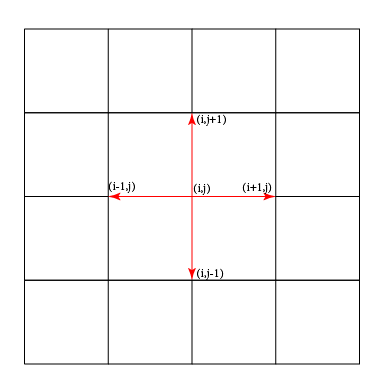
\includegraphics[scale=0.8]{SqLattice.png}
\caption{最近邻hopping}
\end{figure}\label{figHop}
hopping项中,不在对角线上的项是$c_{i\sigma}^\dagger c_{j\sigma}(i\neq j)$,紧束缚近似仅考虑最近邻的格点之间的行为,考虑二维正方点整,对于(i,j)格点上的电子,共有四个最近邻,如图\ref{figHop}所示.在这里所使用的均是二维点阵的索引,在进行矩阵的构建时,需要将这些二维的索引,转变成基矢中对应的索引.\textbf{举例说明:在(i,j)这个格点上,它所对应的$C^\dagger$中的产生算符的索引为(i-1)*xn + j,这里xn是正方格点在x方向的格点数,同样的yn是在y方向上的格点数.这个索引同样可以表示为(j-1)*yn + i,这就是如果将2维点阵上的点,映射成一维基矢上的换算方法,对于其它形式的算符,也是相同的转换技巧.这里还要说明一点,上面选取的是$C^\dagger$中的一个算符,它转换出来的索引,对应的是哈密顿量矩阵中的行索引,对于$C$中选取的算符,它转换出来的索引则对应的是哈密顿量矩阵中的列索引.}上面就是如何将一对算符(2个算符的组合)写成哈密顿量矩阵中的一个元素的方式,这样就可以初步对矩阵进行填值.在方程(\ref{eqhop})和(\ref{eqsoc})中可以看到,实空间的哈密顿量只是明确的写出了$c^\dagger c$的算符着形式,暂且称它是粒子的算符表示形式,但是由方程($\ref{eq6}$)可以看到,哈密顿量中同样还包括了$cc^\dagger$这种组合形式,称它为空穴,由于研究的是关于超导的问题,平均场近似下的哈密顿量是有粒子空穴对称性的,所以肯定会出现这种空穴型的算符,而上面所说的填值问题都是关于粒子的,并没有提及关于空穴该如何构建其哈密顿量对应的值.可以通过费米子算符的对易关系,将空穴的填值问题与粒子的填值联系到一起.
\begin{equation}
\{c^\dagger_i,c_j\}=c^\dagger_ic_j+c_jc^\dagger_i=0
\end{equation}
所以可以得到空穴和粒子的联系是
\begin{equation}
c_jc^\dagger_i=-(c_j^\dagger c_i)^\dagger
\end{equation}
所以只要知道了电子$c_j^\dagger c_i$的填值,将其共轭之后再添负号就是$c_jc_i^\dagger$的填值.再次强调,这里的ij是基矢的索引,而不是二维晶格的直角索引坐标,是它门的2维坐标转换成1维的基矢之后的索引.到这里就将哈密顿量中所有关于最近邻格点之间的项全部介绍完了,而剩下的不过是不同spin以及产生湮灭算符之间的组合,它们涉及到的是分块矩阵之间的组合,这个可以和最近邻矩阵元构建的过程相类比,就可以得到结果.

下面将上述内容具体化:\\
(1,1)block:  ham(m,m+1)   ham(m,m-1)   ham(m,m+xn)   ham(m,m-xn)\\
(2,2)block: ham(xn*yn+m,xn*yn+m+1)   ham(xn*yn+m,xn*yn+m-1)   ham(xn*yn+m,xn*yn+m+xn)   ham(xn*yn+m,xn*yn+m-xn)\\
(3,3)block和(4,4)block的操作与上面的平移类似
\begin{figure}[h]
	\centering
	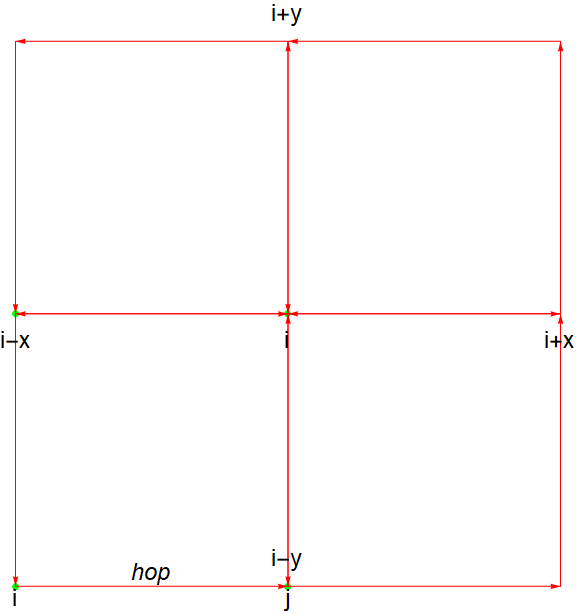
\includegraphics[scale=0.6]{lattice.png}
\end{figure}
\subsection{pari项矩阵填充}
(3,1)block:  ham(m,xn*yn*2+m+1)   ham(m,xn*yn*2+m-1)   ham(m,xn*yn*2+m+xn) ham(m,xn*yn*2+m-xn)

\section{周期性边界问题}
\begin{figure}[h]
	\centering
	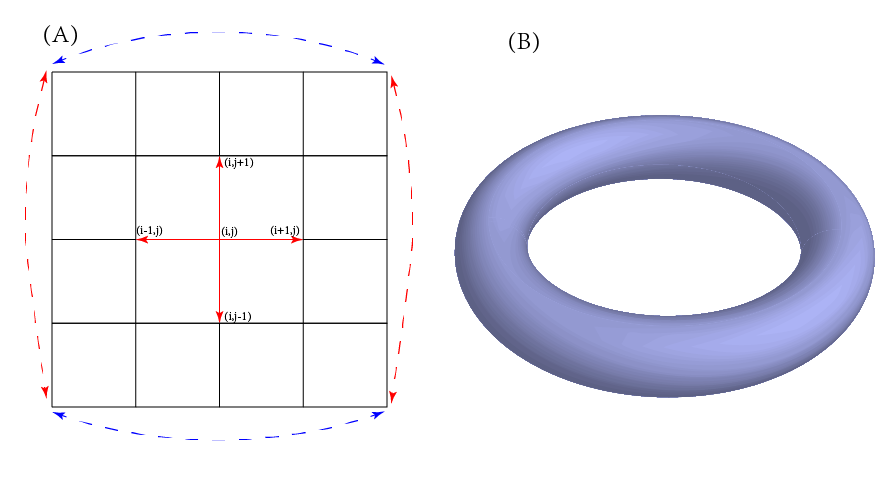
\includegraphics[scale=0.6]{periodic.png}
\end{figure}











\includepdf[pages=2]{file/prb.pdf}	
\end{document}